\documentclass{amsart}
\usepackage{amssymb, amsmath, amsthm, enumitem, siunitx,graphicx}
\usepackage{mathabx}
\usepackage{listings}
\usepackage{hyperref}
\usepackage{cite}
\theoremstyle{definition}
\newtheorem{prb}{Problem}
\lstdefinestyle{code} {
  mathescape,
  columns=fullflexible,
  basicstyle=\fontfamily{lmvtt}\selectfont,
  language=python,
}

\begin{document}
\title{6.S083 Final Project: \\Generative music with N-Grams}
\author{Trevor Henderson}
\date{\today}
\maketitle

\section{Introduction}

The goal of my project is to make a system that generates music using N-gram models.
There are plenty of generative music systems out there and many of them are based on similar theories \cite{prevProject},
however most of them work by analyzing MIDI files to detect predefined patterns like chords and scales.
%chords and scales or the strict rules of baroque counterpoint.
Such systems do a good job of making music that adheres to the genre they are designed to produce, 
but they falter when faced with other genres.
And with so much knowledge built in, it is hard to tell whether or not the quality 
of the resulting music 
is tied to any learning that these systems do.
It could be that regardless of what the system is trained on, the output will sound like real music because it has been forced to follow some basic rules of harmony.
%I believe that while a set of rules is helpful in creating music, it is not the rules in particular the listener hears. 
My goal was to make a more generalized system that does not assume any a priori knowledge of music theory.
In addition, I wanted my system to function by taking a raw audio file as its input, rather than MIDI, and to produce an output song by recombining the source material.
These changes makes the process much more flexible and open to a variety of genres. 
And by using actual audio samples rather than MIDI instruments the music produced can inherit some of the more subtle human qualities from the source which can help keep the music from being overly artificial.

Since, my system has no prior knowledge of music theory and I do not have the resources to train it on the hours of music that would be needed to teach it music theory, my goal with this project is not to produce technically correct music, but rather to produce music that captures the affect of the source material well enough to disguise it as real music from a distance.
This particular quality makes the system well suited for an N-Gram model.
We have seen that sentences created using N-Grams make little to no sense on their own (unless of course $N$ is set large enough for them to be an exact replication of the source).
However, if you were to read only small groups of words at a time 
or to read without 
critically thinking about the meaning of the words 
%which might happen if the you were glancing over a page
, N-Gram sentences can be disguised as real English. 
Similarly, the music produced by my system might come off as strange to any trained ear,
but when it is slightly out of focus as in the case of background music, it acts as a decent impersonator.

% written in C++

\newpage

\section{Steps}

\subsection{Overview}

My system works as follows:
\begin{enumerate}[label=\arabic*.]
  \item
    The input audio source is broken up into individual note samples.
  \item
    Each note is mapped to a list of notes with similar harmonic content.
  \item
    A list of notes is composed one at a time by randomly picking from a pool of potential notes. 
    The pool is determined based on $N-1$ previously chosen notes where $N$ is the order of the N-Gram model.
    %This pool of potential notes is a list of all of the notes whose $N-1$ predecessors in the source material
    %have similar harmonic content to the previous $N-1$ notes added to the song. 
    %Here, $N$ is the order of the $N$-gram.
  \item
    A list of values representing the volume at which each note should be played at is also generated using an $N$-gram model.
  \item
    The pitch and dynamics information are combined together in a full song.
  \item
    The audio samples are stitched together
    and the result is written to file.
\end{enumerate}

\subsection{Onset Detection}

I use the term ``notes'' in a general sense to mean notes, chords, and any sort of individual element in a song.
These notes act like words in an N-gram and form the building blocks in making musical sentences.
Breaking a song into notes is a well studied and still fairly open problem called ``Onset Detection.''
The main challenge of onset detection is to design some sort of function that maps each sample of an audio file
to a value representing the amount of musical change associated with that sample.
A simple function could just measure the relative change in amplitude between groups of samples, 
however more complicated ones attempt to measure changes in harmonic content.
Since such functions have been fine tuned and optimized over the years by researchers,
I decided it would be better to use an external library for this rather than implementing it myself.
I am using the {\sc ComplexODF} function from John Glover's library 
\href{https://github.com/johnglover/modal}{modal}
\cite{modal}.

With an onset detection function in place, finding the onsets is an easier task of choosing each sample where there is a peak in that sample's function value.
My peak finding algorithm divides the audio up into slices no smaller than 20 milliseconds 
which is the smallest time interval that most people can hear.
I've plotted the detected onsets with a small sample from the Aria of Bach's Goldberg Variations below:

{\centering
\begin{center}
  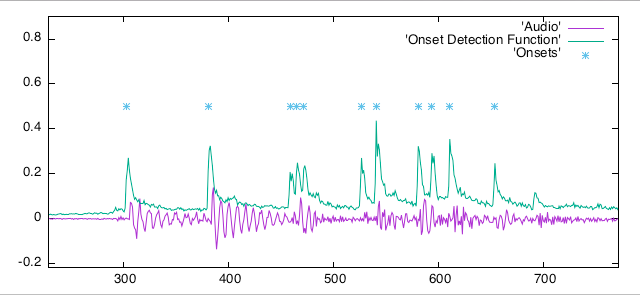
\includegraphics[scale = 0.3]{onsetPlot}
  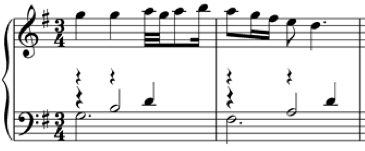
\includegraphics[scale = 0.5]{sheetMusic}
\end{center}
}

From the graph and score of the same 2 measure phrase, we can see that the algorithm detected every note except for the last quarter note in the bass clef, which is played particularly softly and comes below the noise threshold that I've set.
Because my algorithm can handle polyphony, small phrases work fine with the rest of the algorithm.

\subsection{Harmonic Comparison}

After a song is divided into individual notes, each note is compared with every other note
in order to map their harmonic similarities.
The harmonic content of each note can be obtained by taking the Fourier transform of the samples representing that note.
Ideally, 
we could just take the normalized dot product between the transforms, 
however this leads to several problems.
Since the notes come in all sorts of lengths, their transforms are generally not of the same size.
Additionally, in polyphonic music, the exact repetition of a particular chord voicing is rare, which makes the data sparse.
To solve both of these problems, my solution was to map every transform to a constant sized array
representing one octave of frequencies. 
All frequency components in the original transform are mapped to their harmonic equivalent within this octave.
By doing this I am making the assumption that notes have the same harmonic meaning
no matter what octave they are played in,
which I believe is generally fair in the context of most western music.
For simplicity I chose to map all notes to the octave between $1$ and 2 Hertz and 
I made the corresponding array of size 60
which is equally divisible by the number of semitones in an octave (12).
Therefore if a bin of a notes transform represents frequency $f$, I map it to a bin 
%\begin{align*}
$
  60\cdot(\log_2 f \pmod 1)
$
%\end{align*}
of the octave-spectrum.

The bin frequencies in a discrete Fourier transform are linearly space,
therefore this mapping produces a bias in the output to the lower half of the octave.
Also, the resolution of a Fourier transform is not fine enough to distinguish frequency components that lie between different bins.
I implemented a frequency estimation algorithm as described in a paper by Barry G. Quinn\cite{freqEst} to solve these problems.
With these methods in place,
I define the harmonic similarity between two notes as the
normalized dot product between each note's octave-spectrum.

I used a virtual piano to create an audio file with 4 chords: $C$, $C$, $C$, and $C\#m$ voiced as follows:

{\centering
\begin{center}
  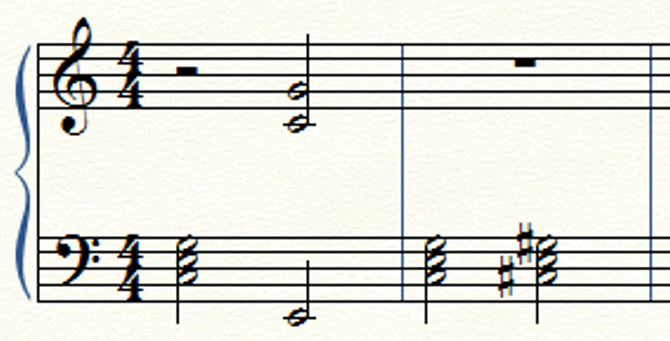
\includegraphics[scale = 0.5]{chords}
\end{center}
}

The corresponding octave-spectrum for the first two chords is:

{\centering
\begin{center}
  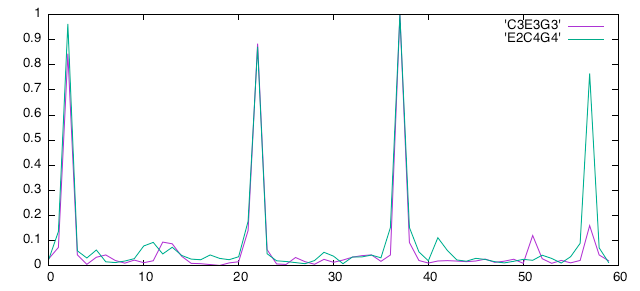
\includegraphics[scale = 0.4]{sameChord}
\end{center}
}

Even though these two $C$ chords are voiced differently, they appear almost the same in the spectrogram.
However there is an extra spike in the second chord towards the end of the spectrum, which corresponds to the note $B$ which is not in the chord.
On a piano, lower notes have more resonant overtone series so the $B$ arises from being the fifth of the low note $E$.
Although its not written in the score, this note is audible to most listeners.
Despite this, the calculated correlation between these two chords is $0.93$.

The second pair of chords, a $C$ and a $C\#$, have the note $E$ in common, but the root and fifth of the chords differ by a semitone.
The octave-spectrum of both chords is:

{\centering
\begin{center}
  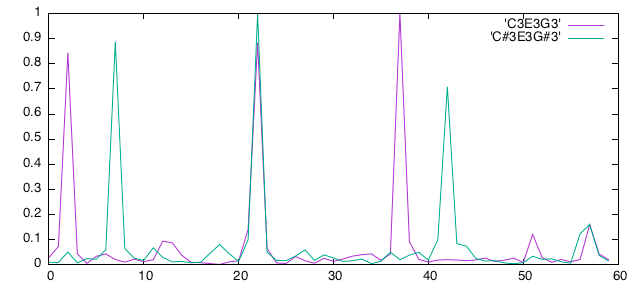
\includegraphics[scale = 0.4]{difChord}
\end{center}
}

Here the harmonic correlation between the two chords is 0.42.
In general I have found a good threshold for harmonic similarity to be 0.8.

\subsection{N-Grams}

After the notes have been grouped, it is time to generate music!
I have set up the program so that output songs must start and end like the source material
which gives the impression that the output audio is some sort of improvisation on the source.
For the rest of the song, I use an N-Gram model to generate notes.
Because my data is small I decided that rather than calculating probability associations between each note,
it would be easier to pick randomly from a pool of potential notes at each step.
For example, suppose I was using a bi-gram model and the input song included more $C$ to $B$ transitions then $C$ to $D$ transitions.
If the last note I chose for my song was a $C$, then the pool of potential notes will include more $B$ notes than $D$ notes,
making the $B$ transitions more likely.

I create this pool by finding all notes whose $N - 1$ predecessors are harmonically similar to the previous $N - 1$ notes added to the song. 
For pitch, I have found $N = 3$ to have the best results. The output is not too random to lose its musicality and not too similar to the source audio.

After I have generated pitch information using N-Grams, I generate dynamic information as well.
After some initial testing with just a pitch based N-Gram I realized that the volume would jump up and down as the system
went back and forth between choosing notes in the soft and loud parts of a song.
With generated dynamic information, the output volume flows more like natural music.
Here my metric of similarity is the ratio between the peak amplitudes of two notes.
I have found that a dynamic threshold of $0.9$ and an N-gram order of $N = 4$ to work well for this.

\subsection{Post-processing}

After the pitch and dynamic information has been generated, all thats left to be done is to put it all together.
I scale the samples of each note in order for it to have the desired volume.
In order to avoid clicks between each pair of notes, I add a small crossfade of 1 millisecond between adjacent notes.
Up until this point all of the sound analysis I have done has been based solely on the left channel of the audio, 
but for realism I write the output in stereo.
The result is written to a wav file.

\section{Results}

To test my my code I added an output parameter which measures the originality of the new piece of music.
It measures the ratio of note transitions in the generated song that were not present in the original song,
to the number of total number of note transitions in the generated song.
For slow and simple songs, this value tended to be around $80\%$, while for 
faster and more complicated songs it went as low as 30\%.
Generally I found that instruments with sharp attack like pianos and guitars tended to have better results than more flowing
brass and string instruments where onsets are difficult to detect.
In faster songs each new note is played while others are still ringing,
which makes each note more harmonically complex and therefore harder to match to other notes.

I have posted a number of pieces that I generated using this code to 
\href{https://soundcloud.com/user-12541400}{Soundcloud}.
My favorite of them is based on Erik Satie's impressionist piece 
\href{https://soundcloud.com/user-12541400/gymnopedie-no1}{Gynopedie No. 1}.
I also generated a variation of each of Bach's 
\href{https://soundcloud.com/user-12541400/sets/goldberg-variations-variations}{Goldberg Variations}.
In addition to some other more serious examples, I've also tried the system on some more complicated genres including 
including hip-hop, electronic music, and
\href{https://soundcloud.com/user-12541400/carry-on-wayward-son}{dad rock}
with amusing results.

%%%%%%%%%%%%%

\section{Usage}

My source code and a compiled executable are available on 
\href{
https://github.com/sportdeath/N-Gram-Music
}{Github}.
The code is written in C++.
I have only ever tested my code on OSX, however I believe it should run on any unix based system.
The code depends on two external libraries: 
\href{http://www.mega-nerd.com/libsndfile/}{libSndFile}\cite{libSndFile}
, which does basic reading and writing of audio files
and
\href{http://www.fftw.org}{FFTW}\cite{fftw}, an efficient fast fourier transform library developed at MIT, which I used for frequency analysis.

Both libraries are available through
\href{http://brew.sh}{Homebrew},
a popular package manager for OSX, or they can be compiled from source.
To install them through brew, run

\begin{lstlisting}[style=code]
    $\text{\$}$ brew install libSndFile fftw
\end{lstlisting}

To run the code, navigate to the directory that you downloaded from github. 
3 test songs are included with the code in a zip file, which you should unzip.
My code is only designed to accept ``.wav'' files, so if you would like to run 
the code on your own music you can convert it to wav using the music file converter
\href{http://sourceforge.net/projects/xld/}{XLD}. 
To create an improvisation run the following command:

\begin{lstlisting}[style=code]
    $\text{\$}$ ./n-gram-music  ``testSong.wav''
\end{lstlisting}

``testSong.wav'' should be the directory of the input song. 
This will create an improvisation and write it to ``testSong-n-gram.wav''.
10 different songs are actually generated and the one closest to 2 minutes long is chosen in order to avoid making songs that are too short or too long.
Other valid arguments include 
\begin{lstlisting}[style=code]
    $\text{\$}$ ./n-gram-music  ``testSong.wav'' ``outputSong.wav''
    $\text{\$}$ ./n-gram-music  ``testSong.wav'' ``outputSong.wav'' N-pitch N-dynamics desiredTime
\end{lstlisting}

``outputSong.wav'' should point to the desired output location. ``N-pitch'' and ``N-dynamics'' should be positive integers, representing $N$ in the pitch and dynamics N-grams respectively. If $\text{N-dynamics}\leq 0$ the dynamics N-Gram will be suppressed and the volume of every note in the output will be the same as the volume of that note in the input. 
If ``desiredTime'' is set, the output song will be approximately desiredTime-minutes long.
If $\text{desiredTime}\leq 0$, the output song will be approximately the same length as the input song.

%%%%%%%%%%%%%%%%%%%%%

\section{Future Development}

\subsection{Digital Artifacts}

While my method does what I set out for it to do, there are some caveats. 
By listening to some different results, it is clear that there are digital artifacts.
Part of this has to do with the sound reconstruction.
The only post processing I do is a small cross fade between notes.
On instruments like piano this is not as noticeable, but on stringed instruments, the audio can sound choppy.
By spending more time with the project, I think it would be possible to reduce these artifacts further.
Also, when the system generates dynamics, sometimes particularly soft notes are amplified so much that the noise in the audio file becomes present.
This can be particularly bad on songs with large dynamic changes.
Adding some sort of correlation between pitch and dynamics rather than generating them in independently might help fix sudden jumps in noise.
%These small changes might be enough to take it out of the uncanny valley where it currently resides.

\subsection{Multiple Input Sources}

I originally intended to make this code work on multiple songs.
The functionality still exists, however after generating songs from multiple sources
I decided against including this feature.
Unless both input songs are very similar the resulting song sounds more like someone switching back and forth between
different radio stations than like actual music.
With just one input song, there seems to be enough material to generate original music.

\subsection{Rhythm}

The biggest issue in this project is that I haven't taken into account rhythm.
Rhythm can be particularly hard to understand without a more in depth understanding of the source material.
This understanding would include some sort of information about where the measure divisions lie in a song and where the weak and strong beats should be placed.
I was considering facing this challenge by stretching the length of each note independently of the pitch using spectral decomposition, however this method can sound particularly digital if not implemented correctly.
It turns out for songs without rhythm sections or a strong pulse, the lack of rhythm is not that off-putting. It just sounds more free-form and improvised than written music.

\subsection{Auto-Correction}

I think the best direction for this project to go in, is for these methods to be used as a composition tool rather than for music generation.
N-Grams are used in writing software to provide word suggestions and auto correction.
It would be interesting to parallel this concept with music.
If this system were to be included in a Digital Audio Workstation it could
%see if a system like the one I've developed could be included in a Digital Audio Workstation and provide musicians
provide musicians
with musical suggestions based on their own work and the work of others and to correct small errors.
It might be particularly helpful for electronic musicians writing sample based music to automatically narrow down which samples might work well together without the musician having to manually sift through thousands of audio files.


\newpage

\bibliography{bibliography.bib}{}
\bibliographystyle{plain}


\end{document}
